\documentclass{SKP-beamer}

% --------------------------------------------------- %
%                  Presentation info	              %
% --------------------------------------------------- %
\title[Cloud Computing]{CLOUD COMPUTING}
\subtitle{Cloud Computing - Overview}
\author{PROF.SOUMYA K.GHOSH}
\institute[SIT]{
  SILICON INSTITUTE OF TECHNOLOGY\\
  SAMBALPUR
}
\date{\today}
\logo{
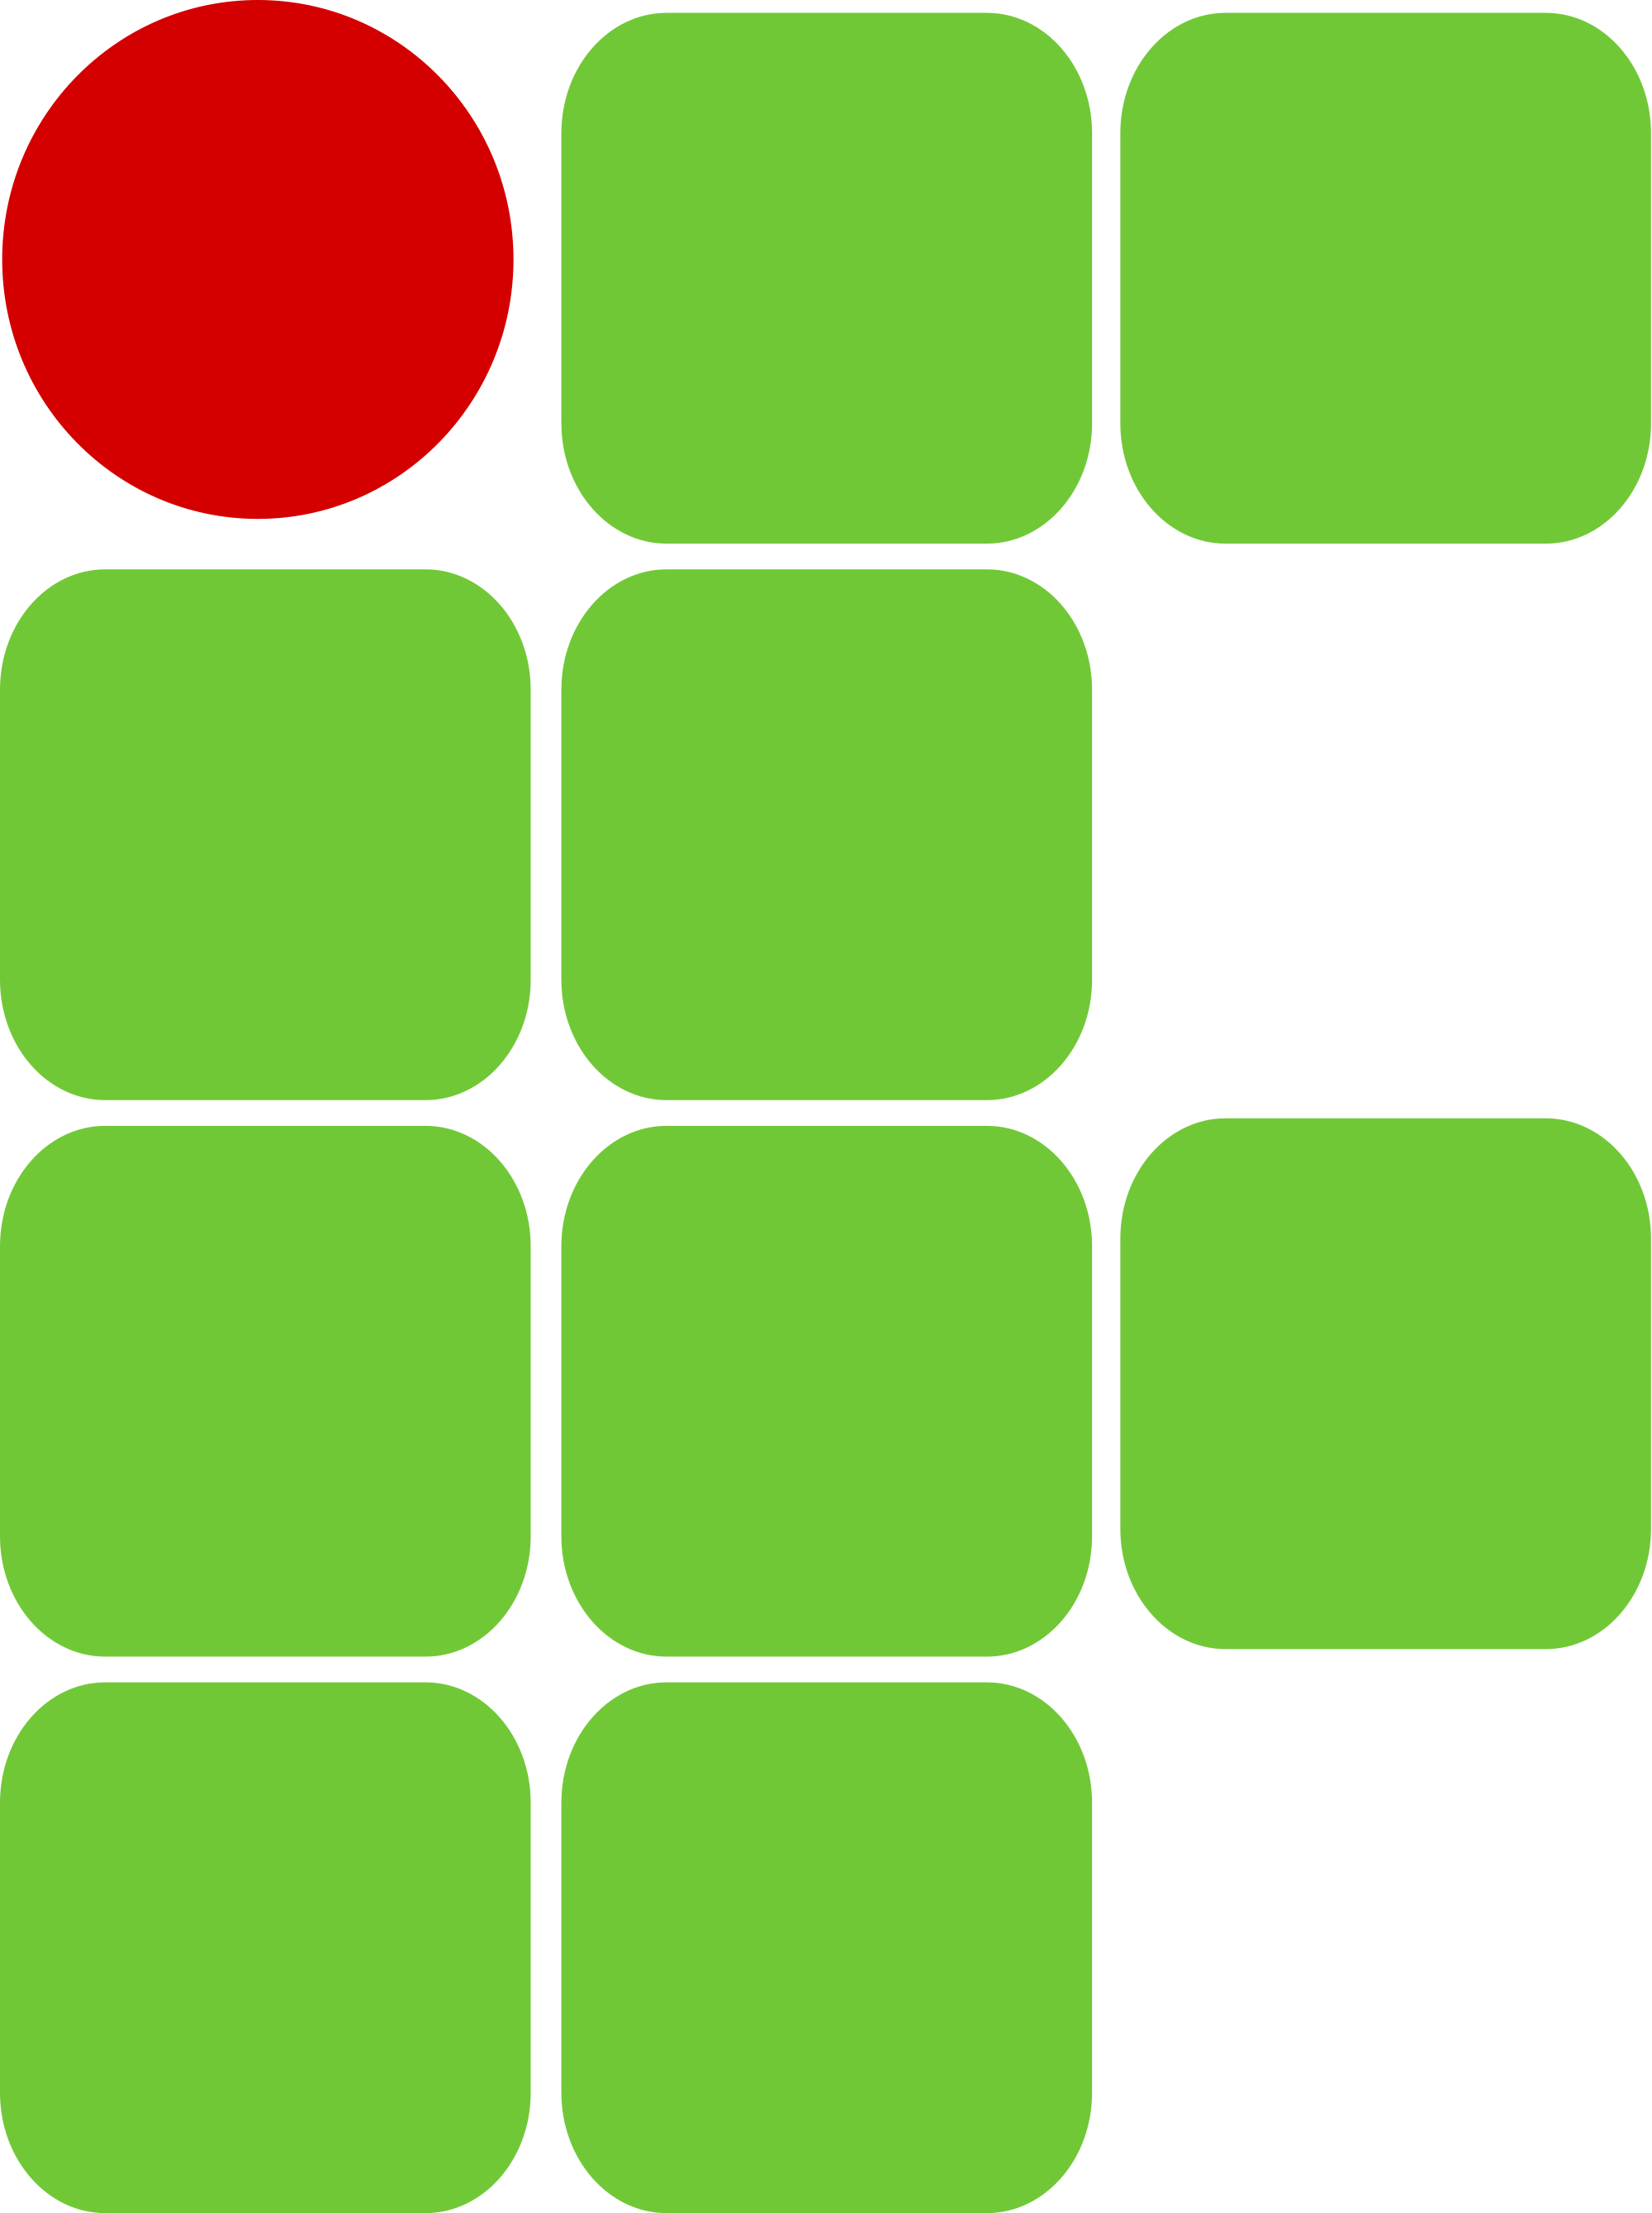
\includegraphics[scale=0.008]{images/logo.png}
}
\subject{Presentation subject} % metadata

% --------------------------------------------------- %
%                    Title + Schedule                 %
% --------------------------------------------------- %

\begin{document}

\begin{frame}
  \titlepage
\end{frame}

\begin{frame}{Introduction}
  The ACM Computing Curricula 2005 defined "computing" as
  
  "In a general way, we can define computing to mean any goal-oriented activity  requiring,  benefiting  from,  or  creating  computers.  Thus, computing includes designing and building hardware and software systems for a wide range of purposes; processing, structuring, and managing various kinds of information; doing scientific studies using computers; making computer systems behave intelligently; creating and  using  communications  and  entertainment  media;  finding  and gathering information relevant to any particular purpose, and so on. The list is virtually endless, and the possibilities are vast."
  
\end{frame}



\begin{frame}{Cloud Computing Course - Overview}
	\begin{itemize}
		\item  Introduction to Cloud Computing
		\begin{itemize}
			\item  Overview of Computing
			\item Cloud Computing (NIST Model)
			\item Properties, Characteristics & Disadvantages
			\item Role of Open Standards
			
		\end{itemize}
		\item Cloud Computing Architecture
			\begin{itemize}
			\item  Cloud computing stack
            \item  Service Models (XaaS)
		        \begin{itemize}
		        	\item  Infrastructure as a Service(IaaS)
		        	\item  Platform as a Service(PaaS)
		        	\item Software as a Service(SaaS)
		        \end{itemize}
			\item  Deployment Models
	    	\end{itemize}
		\item Service Management in Cloud Computing
		        	\begin{itemize}
		        	\item  Service Level Agreements(SLAs)
		        	\item  Cloud Economics
		        	 \end{itemize}
		 \item Resource Management in Cloud 
		 Computing
		 
	\end{itemize}
	
\end{frame}


\begin{frame}{Cloud Computing Course (contd.)}
	\begin{itemize}
		\item  Data Management in Cloud Computing
		\begin{itemize}
			\item  Looking at Data, Scalability & Cloud Services
			\item Database & Data Stores in Cloud
			\item Large Scale Data Processing
		\end{itemize}
		\item Cloud Security
		\begin{itemize}
			\item Infrastructure Security
			\item Data security and Storage
			\item Identity and Access Management
			\item Access Control, Trust, Reputation, Risk
		\end{itemize}
		\item Case Study on Open Source and Commercial Clouds, Cloud Simulator
		\item Research trend in Cloud Computing, Fog Computing
		
		
	\end{itemize}
	
\end{frame}


% --------------------------------------------------- %
%                      Presentation                   %
% --------------------------------------------------- %



\begin{frame}{Trends in Computing}
		\begin{itemize}
		\item Distributed Computing
		\item Grid Computing
		\item Cluster Computing
		\item Utility Computing
		\item \textbf{Cloud Computing}
		
	\end{itemize}
\end{frame}

\section{Distributed Computing}


\begin{frame}{Centralized vs. Distributed Computing}
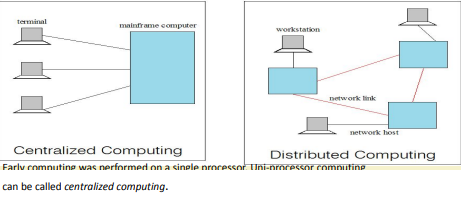
\includegraphics[scale=1.2]{1.png}
\end{frame}


\begin{frame}{Distributed Computing/System?}
	\begin{itemize}
		\item Distributed Computing
		\begin{itemize}
			\item  Field of computing science that studies distributed system
			\item Use of distributed systems to solve computational problems.		
		\end{itemize}
		\item Distributed Computing
		\begin{itemize}
			\item Wikipedia
			
			\begin{itemize}
				\item  There are several autonomous computational entities, 
				each of which has its own local memory.
				\item The entities communicate with each other by message 
				passing.		
			\end{itemize}		
			
			\item Operating System Concept
				\begin{itemize}
				\item The processors communicate with one another through various 
				communication lines, such as high-speed buses or telephone 
				lines.
				\item Each processor has its own local memory.		
			\end{itemize}
		\end{itemize}
		
		
	\end{itemize}
	
	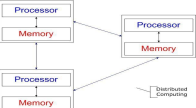
\includegraphics[scale=1.2]{2.png}
	
\end{frame}


\begin{frame}{Example Distributed Systems}
	\begin{itemize}
		\item Internet
		\item ATM(bank) machines
		\item Intranets/Workgroups
		\item Computing landscape will soon consist of 
		ubiquitous network-connected devices
		
		
	\end{itemize}
\end{frame}


\begin{frame}{Computers in a Distributed System}
	\begin{itemize}
		\item Workstations : Computers used by end-users to perform 
		computing
		\item Server Systems: Computers which provide resources and
		services
		\item Intranets/Workgroups
		\item Personal Assistance Devices: Handheld computers connected to the system via a wireless communication link.
		
	\end{itemize}
\end{frame}

\begin{frame}{Common properties of Distributed Computing}
	\begin{itemize}
		\item Fault tolerance
		\begin{itemize}
			\item  When one or some nodes fails, the whole system can still work fine except performance.
			\item Need to check the status of each node
		\end{itemize}
		\item Each node play partial role
		\begin{itemize}
			\item Each computer has only a limited, incomplete view of the system
			\item Each computer may know only one part of the input.
		\end{itemize}
		\item Resource sharing
		\begin{itemize}
			\item Each user can share the computing power and storage resource in the system with other 
			users
		\end{itemize}
		\item Load Sharing
			\begin{itemize}
			\item Dispatching several tasks to each nodes can help share loading to the whole system.
		\end{itemize}
		\item Easy to expand
		\begin{itemize}
			\item We expect to use few time when adding nodes. Hope to spend no time if possible.
		\end{itemize}
		\item Performance
		\begin{itemize}
			\item Parallel computing can be considered a subset of distributed computing.
		\end{itemize}
	\end{itemize}
	
\end{frame}


\begin{frame}{Why Distributed Computing?}
	\begin{itemize}
		\item Nature of application
		\item Performance
		
	
         	-- Computing Intensive
		\begin{itemize}
		\item The task could consume a lot of time on computing. For 
		example, Computation of Pi value using Monte Carlo simulation
	\end{itemize}
	       -- Data Intensive
	       \begin{itemize}
	       	\item The task that deals with a large amount or large size of files. For 
	       	example, Facebook, LHC(Large Hadron Collider) experimental data 
	       	processing.
	       \end{itemize}
	     \item Robustness \\
	       -- No SPOF (Single Point Of Failure)\\
	       -- Other nodes can execute the same task executed on failed 
	       node.
	       
    \end{itemize}
\end{frame}


\section{\textbf{THANK YOU!!}}

\begin{frame}
	\titlepage
\end{frame}


\begin{frame}{Why Distributed Computing?}
	\begin{itemize}
		\item Nature of application
		\item Performance
		
		
		-- Computing Intensive
		\begin{itemize}
			\item The task could consume a lot of time on computing. For 
			example, Computation of Pi value using Monte Carlo simulation
		\end{itemize}
		-- Data Intensive
		\begin{itemize}
			\item The task that deals with a large amount or large size of files. For 
			example, Facebook, LHC(Large Hadron Collider) experimental data 
			processing.
		\end{itemize}
		\item Robustness \\
		-- No SPOF (Single Point Of Failure)\\
		-- Other nodes can execute the same task executed on failed 
		node.
		
	\end{itemize}
\end{frame}


\begin{frame}{Distributed applications}
	\begin{itemize}
		\item Applications that consist of a set of processes that are distributed across a 
		network of machines and work together as an ensemble to solve a 
		common problem
		\item In the past, mostly “client-server”
		\begin{itemize}
			\item Resource management centralized at the server
		\end{itemize}
		
		\item “Peer to Peer” computing represents a movement towards more “truly”
		distributed applications
		
		
		
	\end{itemize}
\end{frame}

\begin{frame}{Clients invoke individual servers}
	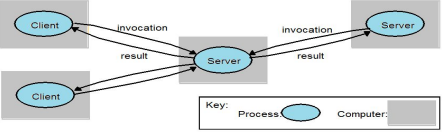
\includegraphics[scale=1.2]{3.png}
\end{frame}


\begin{frame}{A typical distributed application based on peer processes}
	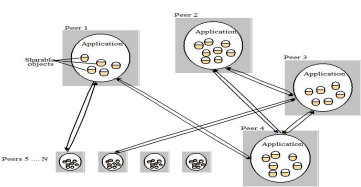
\includegraphics[scale=1.4]{4.png}
\end{frame}


\section{\textbf{Grid Computing}}

\begin{frame}{Grid Computing?}
	\begin{itemize}
		\item Pcwebopedia.com \\
		 – A form of networking. unlike conventional networks that focus on communication 
		among devices, grid computing harnesses unused processing cycles of all computers in 
		a network for solving problems too intensive for any stand-alone machine.
		
		\item IBM \\
		– Grid computing enables the virtualization of distributed computing and data resources 
		such as processing, network bandwidth and storage capacity to create a single system 
		image, granting users and applications seamless access to vast IT capabilities. Just as 
		an Internet user views a unified instance of content via the Web, a grid user essentially 
		sees a single, large virtual computer.
		
		
		\item Sun Microsystems \\
		
		– Grid Computing is a computing infrastructure that provides dependable, 
		consistent, pervasive and inexpensive access to computational capabilities
		
		
		
	\end{itemize}
\end{frame}


\begin{frame}{Grid Computing}
	\begin{enumerate}
		
		\item  Share more than information: Data, computing power, applications in 
		dynamic environment, multi-institutional, virtual organizations \\
		\item  Efficient use of resources at many institutes. People from many institutions
		working to solve a common problem (virtual organisation). \\
		\item  Join local communities. \\
		\item  Interactions with the underneath layers must be transparent and seamless 
		to the user.
		
	\end{enumerate}
\end{frame}


\begin{frame}{ Need Of Grid Computing?}
	\begin{itemize}
		
		\item   Today’s Science/Research is based on computations, data analysis, data 
		visualization & collaborations
		\item Computer Simulations & Modelling are more cost effectivethan
		experimental methods
		\item  JScientific and Engineering problems are becoming more complex & users 
		need more accurate, precise solutions to their problems in shortest possible 
		time
		\item  Data Visualization is becoming very important
		\item Exploiting under utilized resources
		
	\end{itemize}
\end{frame}



\begin{frame}{Who uses Grid Computing ?}
	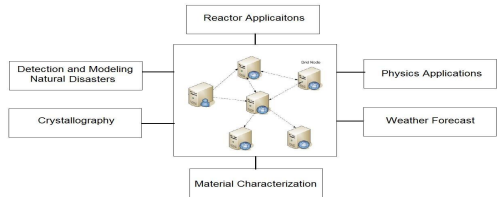
\includegraphics[scale=1.0]{5.png}
\end{frame}

\begin{frame}{ Types Of Grids}
	\begin{itemize}
		
		\item  \textbf{Computational Grid:} These grids provide secure access to huge pool of shared processing 
		power suitable for high throughput applications and computation intensive computing.
		\item \textbf{Data Grid:} Data grids provide an infrastructure to support data storage, data discovery, data 
		handling, data publication, and data manipulation of large volumes of data actually stored 
		in various heterogeneous databases and file systems.
		\item  \textbf{Collaboration Grid:} With the advent of Internet, there has been an increased demand for 
		better collaboration. Such advanced collaboration is possible using the grid. For instance, 
		persons from different companies in a virtual enterprise can work on different components of 
		a CAD project without even disclosing their proprietary technologies
		
	\end{itemize}
\end{frame}

\begin{frame}{}
	\begin{itemize}
		
		\item \textbf{Network Grid:} A Network Grid provides fault-tolerant and high-performance communication 
		services. Each grid node works as a data router between two communication points, 
		providing data-caching and other facilities to speed up the communications between such 
		points.
		
		\item  \textbf{Utility Grid:} This is the ultimate form of the Grid, in which not only data and computation 
		cycles are shared but software or just about any resource is shared. The main services 
		provided through utility grids are software and special equipment. For instance, the 
		applications can be run on one machine and all the users can send their data to be 
		processed to that machine and receive the result back
		
	\end{itemize}
\end{frame}

\begin{frame}{Grid Components}
	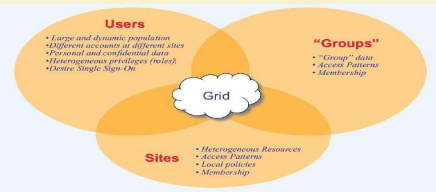
\includegraphics[scale=1.2]{6.png}
\end{frame}


\section{\textbf{Cluster Computing}}



\begin{frame}{What is Cluster Computing?}
	\begin{itemize}
		
		\item   A cluster is a type of parallelor distributed
		computer system, which consists of a
		collection of inter-connected stand-alone computers 
		working together as a single integrated
		computing resource .
		\item Key components of a cluster include multiple 
		standalone computers (PCs, Workstations, or SMPs), 
		operating systems, high-performance interconnects, 
		middleware, parallel programming environments, and
		applications.
		
	\end{itemize}
\end{frame}

\begin{frame}{ Cluster Computing}
	\begin{itemize}
		
		\item   Clusters are usually deployed to improve speed and/or reliability 
		over that provided by a single computer, while typically being 
		much more cost effective than single computer the of comparable 
		speed or reliability
		\item In a typical cluster \\ \\
		– Network: Faster, closer connection than a typical 
		network (LAN) \\
		– Low latency communication protocols \\
		– Loosely coupled than SMP
		
		
		
		
	\end{itemize}
\end{frame}


\begin{frame}{Types of Cluster}
	\begin{itemize}
		
		\item High Availability or Failover Clusters
		\item Load Balancing Cluster
		\item Parallel/Distributed Processing 
		Clusters
		
		
	\end{itemize}
\end{frame}


\begin{frame}{Cluster Components}
	\begin{itemize}
		
		\item Basic building blocks of clusters are broken down into 
		multiple categories :
		\item \textbf{Cluster Nodes}
		\item \textbf{Cluster Network}
		\item \textbf{Network Characterization}
		
			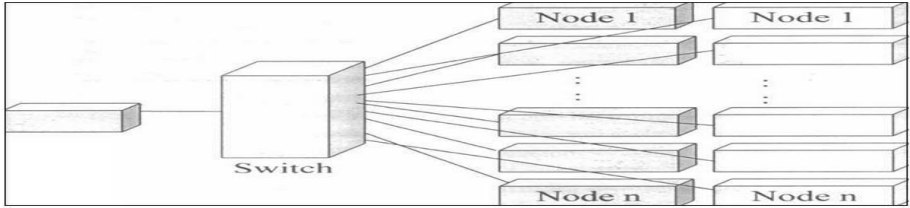
\includegraphics[scale=0.5]{7.png}
		
		
	\end{itemize}
\end{frame}


\begin{frame}{Key Operational Benefits of Clustering}
	\begin{itemize}
		
		\item   System availability: offer inherent high system availability due to the redundancy of hardware, operating systems, and applications.
		\item Hardware fault tolerance: redundancy for most system 
		components (eg. disk-RAID), including both hardware and 
		software.
		\item OS and application reliability: run multiple copies of the OS	and applications, and through this redundancy
		\item Scalability. adding servers to the cluster or by adding more clusters to the network as the need arises or CPU to SMP.
		
	\end{itemize}
\end{frame}

\section{\textbf{Utility Computing}}

\begin{frame}{“Utility” Computing?}
	\begin{itemize}
		
		\item Utility Computing is purely a concept which cloud computing practically implements.
		\item Utility computing is a service provisioning model in which a service provider makes 
		computing resources and infrastructure management available to the customer as 
		needed, and charges them for specific usage rather than a flat rate.
		\item This model has the advantage of a low or no initial cost to acquire computer resources; 
		instead, computational resources are essentially rented.
		\item The word utility is used to make an analogy to other services, such as electrical power, 
		that seek to meet fluctuating customer needs, and charge for the resources based on 
		usage rather than on a flat-rate basis. This approach, sometimes known as pay-per-use
		
		
	\end{itemize}
\end{frame}



\begin{frame}{Utility Computing Example}
	\begin{itemize}
		
		\item On-Demand Cyber
		\item Infrastructure
		
			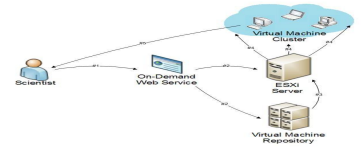
\includegraphics[scale=1.5]{9.png}
		
		
		
	\end{itemize}
\end{frame}

\begin{frame}{Utility Solution – Your 
		Perspective Consumer Provider}
	
		
		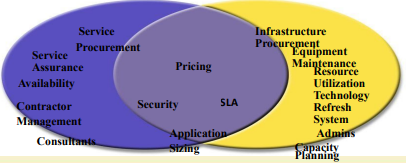
\includegraphics[scale=1.5]{10.png}
		
		
		

\end{frame}



\begin{frame}{ Utility Computing Payment Models}
	\begin{itemize}
		
		\item   Same range of charging models as other utility providers: gas, electricity, telecommunications, water, 
		television broadcasting \\
		 - Flat rate \\
		 - Tiered \\
		 - Subscription \\
		 - Metered \\
		 - Pay as you go \\
		 - Standing charges \\
		\item Different pricing models for different customers based on factors such as scale, commitment and 
		payment frequency
		\item But the principle of utility computing remains
		\item The pricing model is simply an expression by the provider of the costs of provision of the resources and a 
		profit margin
		
		
		
		
		
	\end{itemize}
\end{frame}





\begin{frame}{Overview}

Normal text \alert{Alert Text}  \exemple{Example Text} \emph{Emphasis Text}
\begin{columns}

\begin{column}{0.5\textwidth}

\begin{block}{Simple block}
  \begin{itemize}
  	\item ...
  \end{itemize}
\end{block}

\begin{exampleblock}{Example block}
  \begin{itemize}
  	\item ...
  \end{itemize}
\end{exampleblock}

\begin{alertblock}{Alert block}
  \begin{itemize}
  	\item ...
  \end{itemize}
\end{alertblock}

\end{column}

\begin{column}{0.5\textwidth}

\boxpurple{
\centering
A purple box}

\boxorange{
\centering
An orange box}

\boxgrey{
\centering
A gray box}

\begin{tcolorbox}[tablegreen,tabularx={X||Y|Y|Y|Y||Y}, boxrule=0.5pt, title=My price table]
Color & Price 1  & Price 2  & Price 3 \\\hline\hline
Red   & 10.00   & 20.00   &  30.00 \\\hline
Green    & 20.00   & 30.00   &  40.00  \\\hline
Blue    & 30.00   & 40.00   &  50.00 \\\hline\hline
Orange  & 60.00   & 90.00   & 120.00 
\end{tcolorbox}

\end{column}

\end{columns}
\end{frame}

\section{Cloud Computing}
\subsection{IaaS}
\begin{frame}{Cloud computing}
this is tutorial
\begin{table}[]
	\begin{tabular}{|l|l|l|l|l|l|}
		\hline
		\rowcolor[HTML]{FE0000} 
		dataset    & FABEF     & FABEFOP   & HAREF     & HAREFOP   & RR        \\ \hline
		200 × 20   & 381508.67 & 401105.67 & 166626.67 & 221278    & 902974.67 \\ \hline
		400 × 40   & 447298    & 471459.67 & 198433.67 & 269236    & 1052880.3 \\ \hline
		600 × 60   & 424855.33 & 462263.67 & 196371.67 & 248159.33 & 1130866   \\ \hline
		800 × 80   & 510789.33 & 5374060.7 & 243025    & 305499.67 & 1290577   \\ \hline
		1000 × 100 & 509360    & 550060    & 210131.3  & 314732    & 1411628   \\ \hline
	\end{tabular}
\end{table}
\end{frame}
\begin{frame}{images}
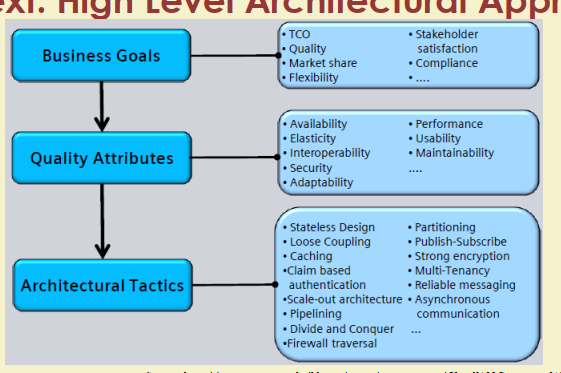
\includegraphics[scale=0.5]{89.png}
\end{frame}


\subsection{PaaS}


\section{Blocks}
\begin{frame}{Blocks types}

\begin{block}{Simple block}
\begin{itemize}
  \item First point
  \item Second point
  \item Third point
\end{itemize}
\end{block}

\begin{exampleblock}{Examples block}
\begin{itemize}
  \item First point
  \item Second point
  \item Third point
\end{itemize}
\end{exampleblock}

\begin{alertblock}{Alert block}
\begin{itemize}
  \item First point
  \item Second point
  \item Third point
\end{itemize}
\end{alertblock}
\end{frame}

\section{Boxes}

\begin{frame}{Boxes}

\boxyellow{
\centering
...}

\boxorange{
\centering
...}

\boxbrown{
\centering
...}

\boxpurple{
\centering
...}

\boxblue{
\centering
...}

\boxgrey{
\centering
...}

\boxgreen{
\centering
...}

\boxblack{
\centering
...}

\end{frame}



\section{Lists}

\subsection{List items}

\begin{frame}{Items}

	\begin{itemize}
		\item ...
    \item ...
    \item ...
  \end{itemize}
  
\end{frame} 

\subsection{Numbered list}

\begin{frame}{Numbered}

	\begin{enumerate}
		\item ...
    \item ...
    \item ...
  \end{enumerate}
  
\end{frame} 

\subsection{Descriptive list} 

\begin{frame}{Descriptive} 

	\begin{description}
		\item [Theme 1:] ...
		\item [Theme 2:] ...
		\item [Theme 3:] ...
	\end{description}

\end{frame}


\section{Tables}

\begin{frame}{Tables 1}

\begin{columns}

  \begin{column}{0.5\textwidth}  

  \begin{tcolorbox}[tablered,tabularx={X||Y|Y}, boxrule=0.5pt, title=My price table]
  Couleur & Prix 1  & Prix 2 \\\hline\hline
  Rouge   & 10.00   & 20.00  \\\hline
  Vert    & 20.00   & 30.00  \\\hline
  Bleu    & 30.00   & 40.00  \\\hline\hline
  Orange  & 60.00   & 90.00 
  \end{tcolorbox}
  
  \begin{tcolorbox}[tableorange,tabularx={X||Y|Y}, boxrule=0.5pt, title=My price table]
  Couleur & Prix 1  & Prix 2 \\\hline\hline
  Rouge   & 10.00   & 20.00  \\\hline
  Vert    & 20.00   & 30.00  \\\hline
  Bleu    & 30.00   & 40.00  \\\hline\hline
  Orange  & 60.00   & 90.00 
  \end{tcolorbox}
  
  \end{column}

  \begin{column}{0.5\textwidth}
  
  \begin{tcolorbox}[tableblue,tabularx={X||Y|Y}, boxrule=0.5pt, title=My price table]
  Couleur & Prix 1  & Prix 2 \\\hline\hline
  Rouge   & 10.00   & 20.00  \\\hline
  Vert    & 20.00   & 30.00  \\\hline
  Bleu    & 30.00   & 40.00  \\\hline\hline
  Orange  & 60.00   & 90.00 
  \end{tcolorbox}
  
  \begin{tcolorbox}[tableyellow,tabularx={X||Y|Y}, boxrule=0.5pt, title=My price table]
  Couleur & Prix 1  & Prix 2 \\\hline\hline
  Rouge   & 10.00   & 20.00  \\\hline
  Vert    & 20.00   & 30.00  \\\hline
  Bleu    & 30.00   & 40.00  \\\hline\hline
  Orange  & 60.00   & 90.00 
  \end{tcolorbox}
  
  \end{column}

\end{columns}
\end{frame}
  
\begin{frame}{Tables 2}
\begin{columns}

  \begin{column}{0.5\textwidth} 
  
  
  \begin{tcolorbox}[tablegrey,tabularx={X||Y|Y}, boxrule=0.5pt, title=My price table]
  Couleur & Prix 1  & Prix 2 \\\hline\hline
  Rouge   & 10.00   & 20.00  \\\hline
  Vert    & 20.00   & 30.00  \\\hline
  Bleu    & 30.00   & 40.00  \\\hline\hline
  Orange  & 60.00   & 90.00 
  \end{tcolorbox}
  
  \begin{tcolorbox}[tablebrown,tabularx={X||Y|Y}, boxrule=0.5pt, title=My price table]
  Couleur & Prix 1  & Prix 2 \\\hline\hline
  Rouge   & 10.00   & 20.00  \\\hline
  Vert    & 20.00   & 30.00  \\\hline
  Bleu    & 30.00   & 40.00  \\\hline\hline
  Orange  & 60.00   & 90.00 
  \end{tcolorbox}

  \end{column}

  \begin{column}{0.5\textwidth}  

  \begin{tcolorbox}[tablepurple,tabularx={X||Y|Y}, boxrule=0.5pt, title=My price table]
  Couleur & Prix 1  & Prix 2 \\\hline\hline
  Rouge   & 10.00   & 20.00  \\\hline
  Vert    & 20.00   & 30.00  \\\hline
  Bleu    & 30.00   & 40.00  \\\hline\hline
  Orange  & 60.00   & 90.00 
  \end{tcolorbox}
  
  \begin{tcolorbox}[tableblack,tabularx={X||Y|Y}, boxrule=0.5pt, title=My price table]
  Couleur & Prix 1  & Prix 2 \\\hline\hline
  Rouge   & 10.00   & 20.00  \\\hline
  Vert    & 20.00   & 30.00  \\\hline
  Bleu    & 30.00   & 40.00  \\\hline\hline
  Orange  & 60.00   & 90.00 
  \end{tcolorbox}
  
  \end{column}

\end{columns}
\end{frame}
  

\section{Figures}

\begin{frame}{Figure Example} 

\begin{figure}
\centering
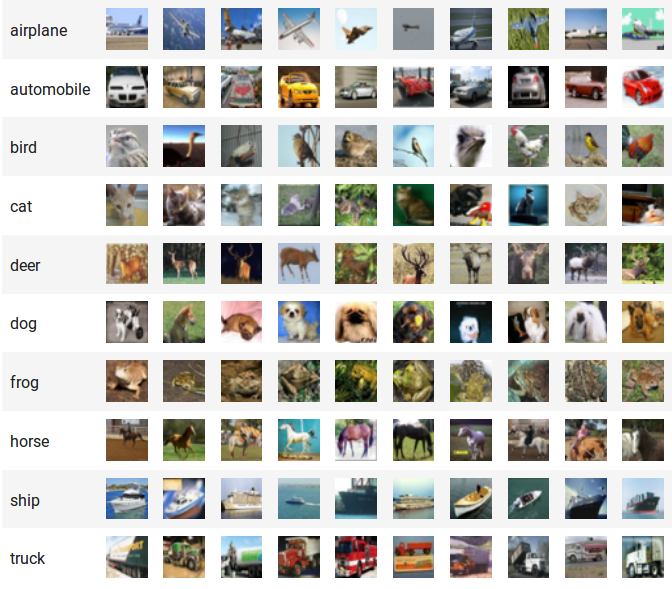
\includegraphics[scale=0.25]{images/cifar10.png}
\caption{Example images from the \href{http://www.cs.toronto.edu/~kriz/cifar.html}{CIFAR-10} dataset.}
\end{figure}

\end{frame}

\section{Equations and Codes}
\subsection{Equations}
\begin{frame}
\frametitle{Equation Example}
Some random equation:

\begin{align*}
    \frac{\partial}{\partial \theta_k}J(\theta) 
        &= \frac{\partial}{\partial \theta_k}\Bigg[\frac{1}{m}\sum_{k=1}^m log(1+e^{-y^{(i)}\theta^Tx^{(i)}})\Bigg] \\
        &= \frac{1}{m}\sum_{k=1}^m \frac{1}{1+e^{-y^{(i)}\theta^Tx^{(i)}}}y^{(i)}x_k^{(i)} \\
        &= -\frac{1}{m}\sum_{k=1}^m h_\theta(-y^{(i)}x^{(i)})y^{(i)}x_k^{(i)}        
\end{align*}

\end{frame}

\subsection{Programming}
\begin{frame}[fragile]

\frametitle{Code Example}

\begin{figure}
\centering
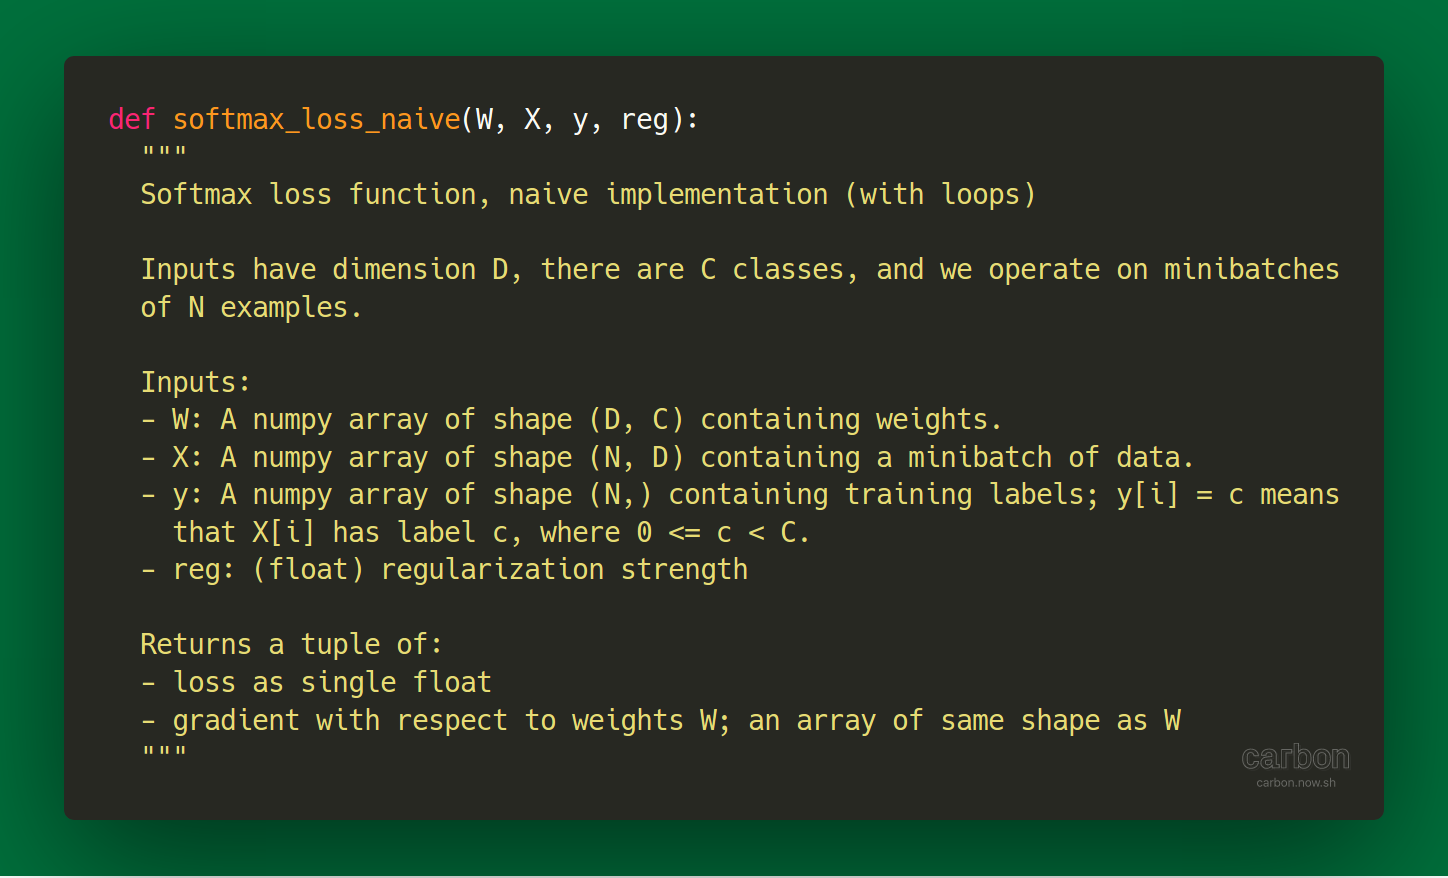
\includegraphics[width=\linewidth]{images/carbon.png}
\end{figure}
\footnote{\href{https://github.com/dawnlabs/carbon}{Carbon}}

% \begin{block}{Code}
% \begin{lstlisting}
% def code():
%   # test comments #1    
%   if True:
%     for _ in range(5):
%       print("Hello World 5 times")
%   return None     
% \end{lstlisting}
% \end{block}

% \begin{lstlisting}[backgroundcolor = \color{lightgray}]
% def code():
%   # test comments #1    
%   if True:
%     for _ in range(5):
%       print("Hello World 5 times")
%   return None     
% \end{lstlisting}

\end{frame}
%%%%%%%%%%%%%%%%%%%%%%%%%%%%%%
\section*{}
\begin{frame}
	\begin{center}
		\begin{pgfpicture}{0cm}{0cm}{3cm}{3cm}
			\pgfmoveto{\pgfxy(3,0)}
			\pgfcurveto{\pgfxy(2,2.2)}{\pgfxy(1,.5)}{\pgforigin}
			\pgfsetlinewidth{2pt}
			\pgfstroke
			
			\pgfmoveto{\pgfxy(0,3)}
			\pgfcurveto{\pgfxy(1,.5)}{\pgfxy(2,2.2)}{\pgfxy(3,3)}
			\pgfstroke
			
			\pgfputlabelrotated{.35}{\pgfxy(0,0)}{\pgfxy(5,3)}{3pt}{\pgfbox[center,base]{\begin{Huge}Thank You!\end{Huge}}}
		\end{pgfpicture}
	\end{center}
\end{frame}
\end{document}
